\clearpage
\onecolumn
\appendix
\section{Идентификация готовых моделей}
\label{app:models}
\begin{table}[!ht]
\centering
\small
\setlength{\tabcolsep}{3pt}
\renewcommand{\arraystretch}{1.18}
\caption{\porozhdeno{\Claim{T03}{Конкретные готовые классификаторы и сведения из записанного происхождения артефактов QIIME. Релиз SILVA указан действием получения референса; релизы GTDB и Greengenes2 устанавливаются только по именам импортов. Источник получения готового файла не следует из источника референсных последовательностей.}}}
\label{tab:models}
\begin{tabular}{@{}p{0.115\textwidth}p{0.11\textwidth}p{0.29\textwidth}p{0.135\textwidth}p{0.29\textwidth}@{}}
\toprule
База & Релиз & Файл модели & Источник готовой модели & Известная подготовка \\
\midrule
SILVA & 138.1, SSURef\_NR99 & \path{silva-138-99-nb-classifier.qza} & URL и автор не установлены & Получение SILVA через RESCRIPt, обратная транскрипция, очистка, фильтрация по длине и дерепликация. \\
\addlinespace
GTDB & r220, по именам импортов & \path{gtdb_classifier_r220.qza} & URL и автор не установлены & Импорт \path{bac120_ssu_reps_r220.fna}, \path{ar53_ssu_reps_r220.fna} и соответствующей таксономии; подготовка до импорта неизвестна. \\
\addlinespace
Greengenes2 & 2024.9, по именам импортов & \path{gg_2024.09.full-length.nb.sklearn-1.4.2.qza} & URL и автор не установлены & Импорт \path{2024.9.backbone.fna} и \path{2024.9.backbone.tax}; подготовка до импорта неизвестна. \\
\bottomrule
\end{tabular}
\end{table}

\porozhdeno{\Claim{M05}{У всех моделей записано обучение действием \texttt{fit\_classifier\_naive\_bayes} в QIIME 2 и \texttt{feature-classifier} версии 2024.5.0; версия \texttt{scikit-learn} --- 1.4.2. Регион последовательностей, праймеры и полнота гена не установлены: слова \texttt{full-length} в имени файла Greengenes2 не являются независимым подтверждением полноты последовательностей. Полные SHA256 однозначно идентифицируют использованные файлы:
\begin{center}
\small
\begin{tabular}{@{}ll@{}}
SILVA & \texttt{c08a1aa4d56b449b511f7215543a43249ae9c54b57491428a7e5548a62613616} \\
GTDB & \texttt{07aadcf7472d9cc6f853f6b4615348619f1a3eceb56c1fb1b6d8dbb20554765f} \\
Greengenes2 & \texttt{5c5900c10ad601b12cf0d2280d52cc0f7852627e89070595cc3899a6d690ee27}
\end{tabular}
\end{center}
}}

\clearpage
\section{Дополнительные знаменатели и причины исключения}
\begin{table}[!ht]
\centering
\small
\caption{\porozhdeno{\Claim{T04}{Разбиение всех ридов образцов Kr после DADA2 по назначениям SILVA: Eukaryota, неизвестный домен, явные метки органелл и оставшиеся прокариотические риды $N$. В этих образцах категории не пересекаются и в сумме дают исходное число ридов; органелльные метки распознаются на любом ранге без учёта регистра. Категории обозначают результат классификации, не независимую проверку биологического происхождения.}}}
\label{tab:krfilter}
\begin{tabular}{lrrrrr}
\toprule
Образец & Всего & Eukaryota & Домен не задан & Органеллы & Осталось \\
\midrule
Kr1\_S80 & 12351 & 9947 & 2364 & 2 & 38 \\
Kr2\_S81 & 8904 & 7780 & 1113 & 11 & 0 \\
Kr3\_S82 & 9985 & 8761 & 1213 & 9 & 2 \\
Kr4\_S83 & 12293 & 10998 & 1046 & 0 & 249 \\
Kr5\_S84 & 1505 & 495 & 1010 & 0 & 0 \\
\bottomrule
\end{tabular}

\end{table}
\begin{table}[!ht]
\centering
\small
\caption{\porozhdeno{\Claim{T05}{Условные знаменатели совпадения полной таксономической линии до рода для каждой почвы и пары моделей: число присутствующих в образце ASV, назначенных обеими моделями, и сумма их ридов. Нулевой знаменатель означает NA; такие образцы не входят в медиану условного совпадения по ридам. Объединённые знаменатели ASV в тексте учитывают каждый уникальный почвенный ASV один раз и не равны сумме столбца по образцам.}}}
\label{tab:conditional}
\begin{tabular}{lrrrrrr}
\toprule
Образец & \multicolumn{2}{c}{SILVA--GTDB} & \multicolumn{2}{c}{SILVA--Greengenes2} & \multicolumn{2}{c}{GTDB--Greengenes2} \\
& ASV & Риды & ASV & Риды & ASV & Риды \\
\midrule
Kr1\_S80 & 0 & 0 & 0 & 0 & 0 & 0 \\
Kr2\_S81 & 0 & 0 & 0 & 0 & 0 & 0 \\
Kr3\_S82 & 0 & 0 & 0 & 0 & 0 & 0 \\
Kr4\_S83 & 1 & 3 & 1 & 3 & 1 & 3 \\
Kr5\_S84 & 0 & 0 & 0 & 0 & 0 & 0 \\
LUB2\_S92 & 297 & 9682 & 326 & 9549 & 244 & 8054 \\
LUB3\_S93 & 167 & 2827 & 183 & 2938 & 136 & 2109 \\
LUB4\_S94 & 300 & 6714 & 336 & 6737 & 248 & 5086 \\
LUB5\_S95 & 290 & 6658 & 315 & 7368 & 206 & 5062 \\
LUB6\_S96 & 407 & 12092 & 437 & 13153 & 321 & 10176 \\
\bottomrule
\end{tabular}

\end{table}
\clearpage
\section{Таксономические профили на уровне семейств}
\begin{figure}[!ht]
\centering
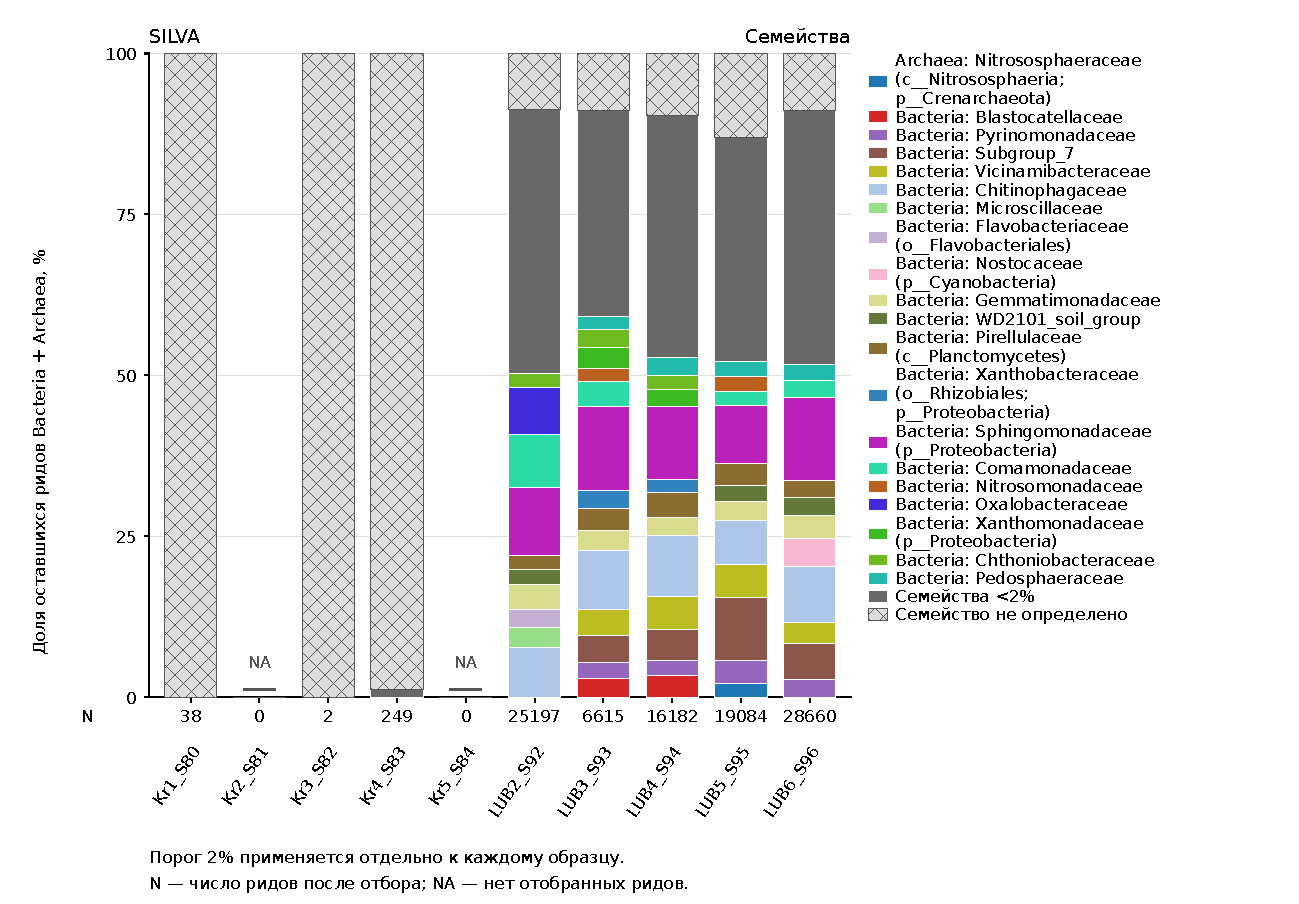
\includegraphics[width=\textwidth]{../../figures/taxonomy/family/prokaryotic_family_silva.pdf}
\caption{\porozhdeno{\Claim{F02}{Таксономические профили на уровне семейств по назначениям модели SILVA. Почвы после модельного отбора Bacteria + Archaea и исключения явно помеченных органелл; знаменатель каждого столбца --- его $N$. \texttt{UNCLASSIFIED} остаётся в знаменателе, точное \texttt{f\_\_uncultured} отнесено к нему; $N=0$ даёт NA. Семейства ниже \SelectedDisplayThresholdPct{}\% данного образца объединены без удаления ридов. Контроль не изображён.}}}
\label{fig:silva}
\end{figure}
\clearpage
\begin{figure}[!ht]
\centering
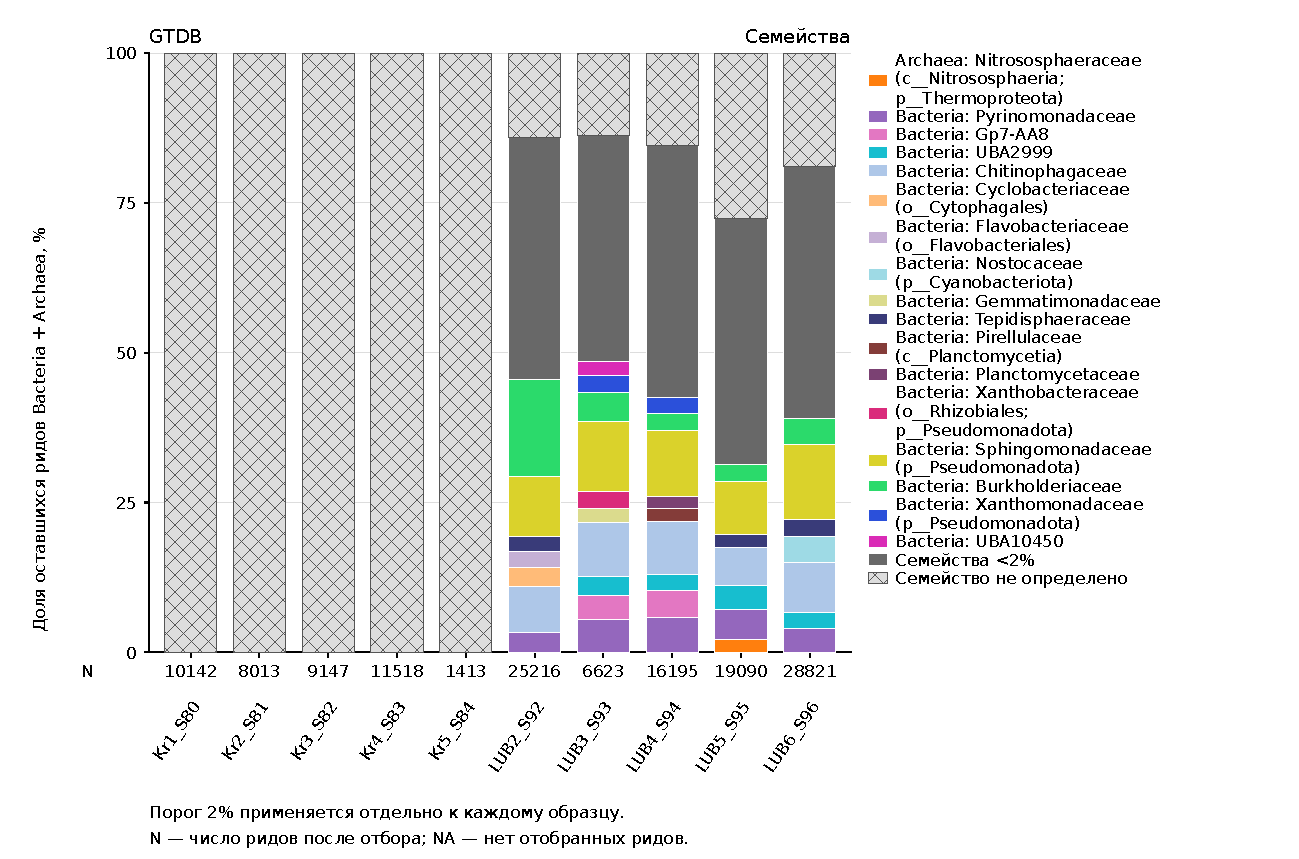
\includegraphics[width=\textwidth]{../../figures/taxonomy/family/prokaryotic_family_gtdb.pdf}
\caption{\porozhdeno{\Claim{F03}{Таксономические профили на уровне семейств по назначениям модели GTDB. Почвы после модельного отбора Bacteria + Archaea и исключения явно помеченных органелл; знаменатель --- собственный $N$ модели. \texttt{UNCLASSIFIED} включает неопределённые семейства и точное \texttt{f\_\_uncultured}; при $N=0$ доля была бы NA. Назначенные семейства ниже \SelectedDisplayThresholdPct{}\% сгруппированы без удаления ридов. Контроль исключён из рисунка.}}}
\label{fig:gtdb}
\end{figure}
\clearpage
\begin{figure}[!ht]
\centering
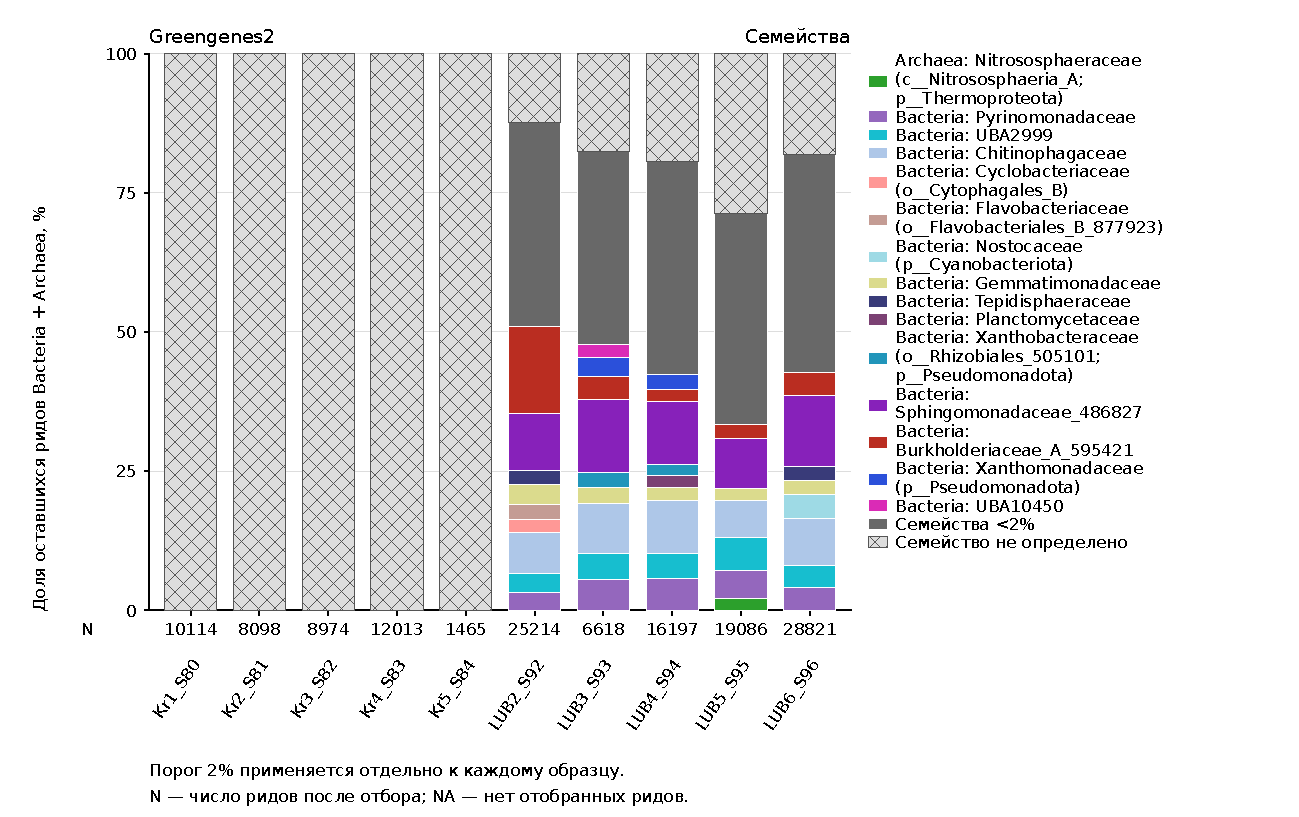
\includegraphics[width=\textwidth]{../../figures/taxonomy/family/prokaryotic_family_gg2.pdf}
\caption{\porozhdeno{\Claim{F04}{Таксономические профили на уровне семейств по назначениям модели Greengenes2. Почвы после модельного отбора Bacteria + Archaea и исключения явно помеченных органелл; знаменатель --- собственный $N$ модели с сохранённым \texttt{UNCLASSIFIED}, включая точное \texttt{f\_\_uncultured}. Пустой отбор означал бы NA. Назначенные семейства ниже \SelectedDisplayThresholdPct{}\% объединены серым, их риды остаются в $N$. Контроль не изображён.}}}
\label{fig:ggtwo}
\end{figure}
